\section{Visual search, object retrieval and person re-identification}\label{sec:visual-search}

\textit{Visual search} principle: given a new image of a specific object or person, find other images relative to the same instance represented in the given one.

Visual search applications:
\begin{myitem}
    \item reverse image search,
    \item web search engine,
    \item personal photo collection,
    \item geolocalization,
    \item query for more information,
    \item shopping interfaces,
    \item ambient intelligence.
\end{myitem}

Main challenges in this task are illumination, object pose, clutter, occlusion, intra-class appearance, viewpoint. Furthermore, the problem is inherently ambiguous: it is very hard to understand what the user means with a single query image, and the user goal is application dependent, thus it is very important to leverage prior information given during training.

Key considerations:
\begin{myitem}
    \item What is the measure of similarity?
    \item How do we represent the image/video?
    \item What is the search procedure?
    \item What background knowledge is available, or what can be learned?
\end{myitem}

The goal of \textit{person search} is to find a queried person within a gallery of images (detection and re-identification). Motivations can range from find missing person to surveillance, to access granting.

Notes:
\begin{myitem}
    \item Detection algorithms find and localize all object instances of a class and all people;
    \item Inference is on unseen object instances and people identities (compare with classification).
\end{myitem}


\subsection{Object Search (or Instance-Level Retrieval)}\label{sec:vs-object}

\textit{Goal}: find specific object instances.

The first problem, when it comes to Object Search, is how to represent objects.\\
\textbf{Early methods} used low-level clues, such as color histograms, texture and shape descriptors. However, they couldn't deal with appearance variation. So, different approaches are necessary.


\subsubsection{Local representations}\label{sec:vs-local}

Local representations leverages on \textbf{local descriptors}, which guarantee invariance by capturing the local appearance, and thus are discriminative; furthermore, they assure repeatability by carefully choosing locations. This approach requires more sophisticated matching, though.\\
The \textit{pipeline} is the following:
\begin{myenum}
    \item Extract local descriptors from the query image,
    \item Compare local descriptors of the query image with local descriptors of each gallery image,
    \item Apply geometric verification to the resulting list of matches,
    \item Return a shorter list of retrieved images.
\end{myenum}
\textbf{Geometric verification}:
\begin{myitem}
    \item From a set of local pairwise matches, find the geometric transformation that fits the highest number of matches,
    \item Retain only images with enough matches for the estimated transformation,
    \item Provides coarse object localization,
    \item Is a costly process, thus we need to verify only a short list of images.
\end{myitem}
There are different approaches to scale the first selection process. On the one hand, efficient approximate nearest neighbor search on local descriptors, using Randomized K-DTrees or Locality-Sensitive-Hashing. On the other hand, \textbf{quantization} of local descriptor space into a visual codebook. That is, discretize the local descriptor space and let two descriptors match if and only if they fall in the same bin. This concept applies to \textbf{Visual Words} (see figure \ref{fig:visual-words}):
\begin{myenum}
    \item Extract some local features from a number of images;
    \item Quantize the feature space, where each point is a descriptor vector;
    \item Map high dimensional descriptors to tokens/words by quantizing the feature space:
    \begin{enumerate}
        \item Quantize via clustering, let cluster centers be the prototype \textit{words};
        \item Determine which word to assign to each new image region by finding the closest cluster center.
    \end{enumerate}
\end{myenum}
To leverage quantization for efficient retrieval, first create an inverted file with all descriptors of the gallery set, then use this for efficiently matching a query image.

\begin{figure}[h!]
    \centering
    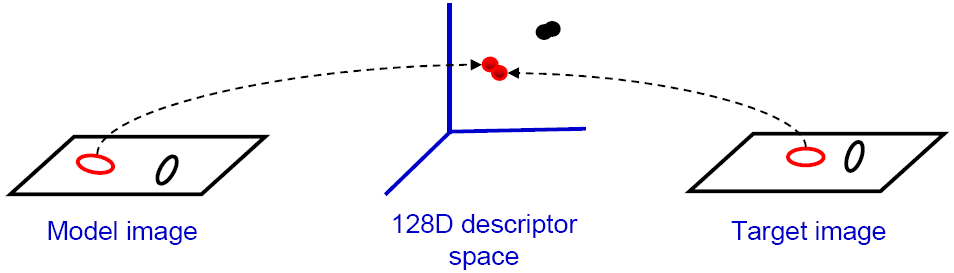
\includegraphics[width=0.7\linewidth]{images/visual-words}
    \caption[Visual Words]{Visual Words}
    \label{fig:visual-words}
\end{figure}


\subsubsection{Global representations}\label{sec:vs-global}

This full pipeline is a costly approach, because of the memory cost of storing all the local descriptors, and the computational cost of matching and verification. Thus, an alternative cheaper approach is to use global representations: \textbf{global descriptors} aggregate individual local descriptors per image, then simple similarity measures can be applied between global descriptors.

An example of this approach is \textbf{Bag of Words}:
\begin{itemize}
    \item Extract local descriptors;
    \item Convert them into visual words, using a visual codebook;
    \item Represent images as histograms of occurrences.
\end{itemize}

In this way, the obtained representation is relatively coarse, thus we can increment the number of entries in the codebook, but with a significant computational cost, or use other statistics, such as mean and variance.
\textbf{Mean: VLAD} (Vector of Locally Aggregated Descriptors)
\begin{myitem}
    \item Aggregate all descriptors assigned to the same visual word;
    \item Concatenate vectors for individual words.
\end{myitem}
\textbf{Mean + Variance: Fisher Vector}
\begin{myitem}
    \item Probabilistic codebook as a mixture of Gaussians;
    \item Descriptors soft assigned to words;
    \item Compute the gradient of the log likelihood with respect to the parameters of the model;
    \item Aggregate the contribution of all local descriptors;
    \item Concatenate statistics for all the visual words.
\end{myitem}

We can use \textbf{mean Average Precision} (mAP) to evaluate those different approaches. The result is that \textit{matching-based methods} (i.e., local representations) give highest accuracy, but with the high cost of matching and geometric verification, while \textit{aggregation methods} (i.e., global representations) are faster and more efficient, but give lower accuracy.

\begin{figure}[h!]
    \centering
    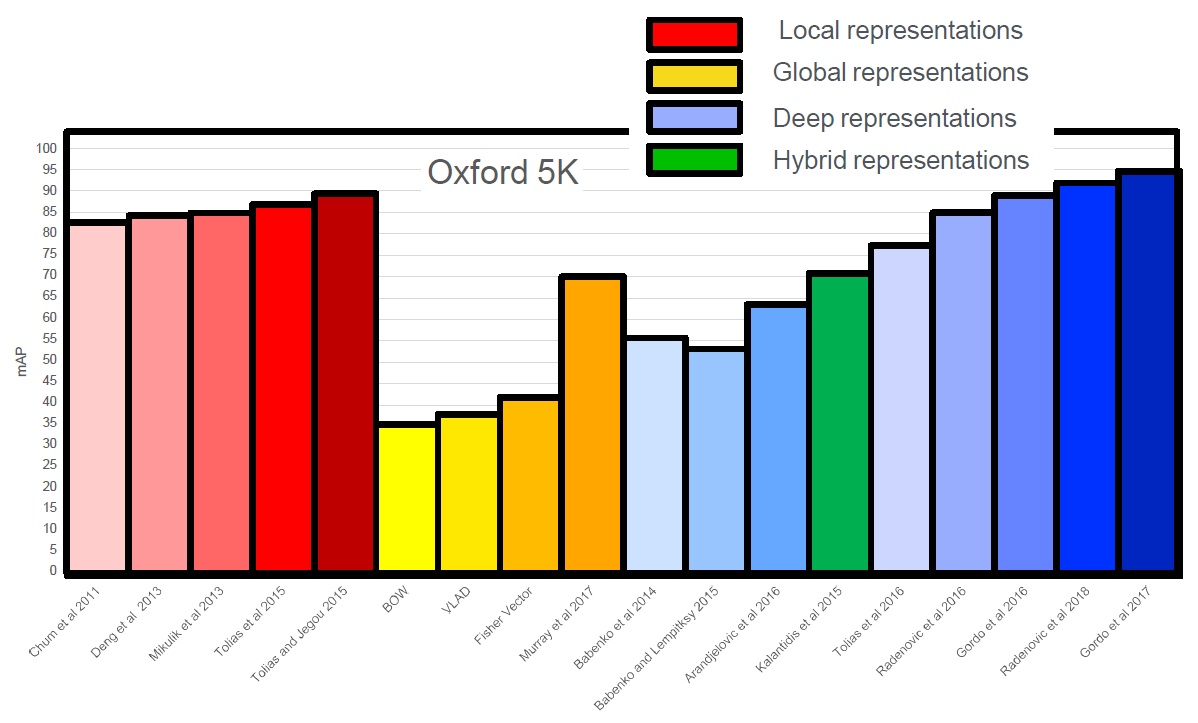
\includegraphics[width=0.9\linewidth]{images/oxford-map}
    \caption[Evaluation of different kinds of representation on Oxford 5K dataset]{Evaluation of different kinds of representation on Oxford 5K dataset}
    \label{fig:oxford-map}
\end{figure}


\subsubsection{Deep representations}\label{sec:vs-deep}

A naive deep learning approach consists in pretraining a network for classification and using it as a feature extractor. The resulting representations are compact and fast at test time. The problem is the network is trained for generic classes (intra-class generalization) and the produced representation has low resolution and distorted aspect ratio, thus leading to underwhelming results.

The first solution is to combine with more standard approaches, that is, \textit{hybrid methods}:
\begin{myitem}
    \item \textbf{CNN + VLAD = NetVlad}: add a VLAD block at the end of a CNN;
    \item \textbf{Fisher Vectors + Fully Connected Layers}: combine some unsupervised for computing low level descriptors with supervised fully connected layers;
\end{myitem}
The second solution is to improve the pipeline to tailor it to the retrieval task, using \textit{recent deep approaches}.
A first approach of this kind, may be to collect and leverage an appropriate training set, and then fine tune the network. But there are some limitations: images are distorted, the network still uses a classification loss, public landmark datasets are noisy. Various aspects can be improved:
\begin{myitem}
    \item \textit{Training data:} automatic cleaning of the landmark images, resulting in less images, but with bounding box annotations;
    \item \textit{Architecture}:
    \begin{itemize}
        \item Small details are important for instance level retrieval: need to accommodate high resolution, undistorted images during training;
        \item Use \textbf{R-MAC descriptor} to obtain local features from input images;
        \item Compute local features using  a CNN, then aggregate them into region feature vectors, and combine them into a final global representation;
        \item Advantages: no aspect ratio distortion, can encode high resolution images, fast comparison with the dot product;
        \item Observations: The aggregation steps can be integrated inside the network, since every step is differentiable, the model can be trained end-to-end;
    \end{itemize}
    \item \textit{Training objective}:
    \begin{itemize}
        \item Train explicitly for retrieval;
        \item To learn to rank, use a network that takes in input three images: the query image, a relevant image and a non relevant image (see figure \ref{fig:training-retrieval});
        \item Use a \textit{triplet loss} which combine information from all the input images:
        \begin{equation}\label{eq:retrieval-triplet-loss}
            L_v(q,d^+,d^-) = \frac12 \max(0, m + \norm{q-d^+}^2 - \norm{q-d^-}^2),
        \end{equation}
        where $q$ is related to the query image, $d^+$ to the relevant image and $d^-$ and $m$ to the non relevant image.
    \end{itemize}
\end{myitem}

\begin{figure}[h!]
    \centering
    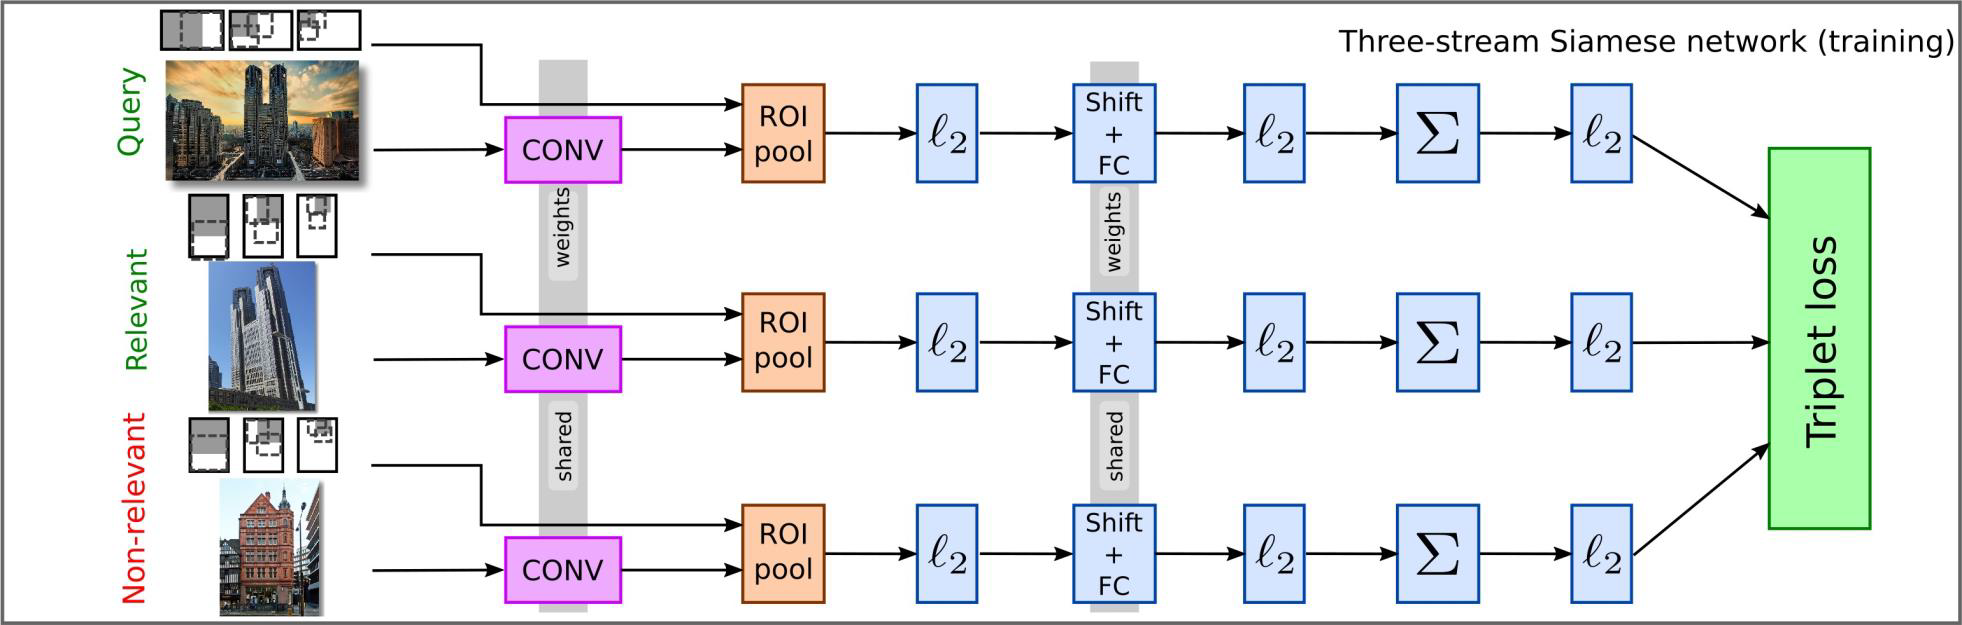
\includegraphics[width=0.7\linewidth]{images/training-retrieval}
    \caption[Training for retrieval]{Training for retrieval}
    \label{fig:training-retrieval}
\end{figure}


\subsection{Person Search}\label{sec:vs-person}

Goal: find specific person identities.


\subsubsection{Person Re-Identification}\label{sec:vs-reidentification}

\textit{Sub-goal}: find the queried person in a gallery of cropped samples. Retrieve the same person from different cameras, assuming that image crops are produced by a person detector.

The datasets for image re-identification are composed of boxes (hand written or obtained from a detector). The boxes in the training set are associated with an identity; the images in the test set represent people not seen at training. Thus, the algorithm should generalize to recognize unseen people from a query.

The re-identification task poses many challenges:
\begin{myitem}
    \item Inaccurate detections;
    \item Large variations of viewpoint and poses;
    \item Large inter id variation, similar appearance of different identities;
    \item Occlusions;
    \item Varying lighting/weather conditions;
    \item Different camera setups and resolutions.
\end{myitem}

There are two main evaluation metrics we can use for re-identification:
\begin{myitem}
    \item \textbf{Cumulative Matching Characteristic}:
    \begin{itemize}
        \item As from object retrieval literature;
        \item Probability that a match will be found in top-k results for a query.
    \end{itemize}
    \item \textbf{Mean Average Precision}:
    \begin{itemize}
        \item Similar to evaluating classification;
        \item Specific emphasis on recall;
        \item A perfect re-identification model should recall all true matches;
        \item Sort the gallery by the score similarity function with respect to a certain query, compute the average precision over the obtained vector, average over all the queries;
        \item Weighted mean of precisions achieved with increasing thresholds.
    \end{itemize}
\end{myitem}

There are many different approaches to person re-identification, but the fundamental points are:
\begin{myitem}
    \item Find representations invariant of pose, viewpoint, illumination...
    \item Fix the alignment issue, using spatial transformer networks, pose estimation/part or joint localization, or attention mechanism.
\end{myitem}

The approaches we discuss are CNN-based:
\begin{myitem}
    \item Perform feature extraction by learning features embeddings, apply identification models and Triplet Loss (see \ref{eq:retrieval-triplet-loss}), then compare identities by their embeddings (obtained from the last fully connected layer of the network).
    \item Use verification models with binary classification loss, that is, a network which takes in input a pair of images, extracts local features separately for each image, then measures similarity with another sub-network, and compute a loss that predicts if the images represent the same person or different persons.
\end{myitem}
A simple \textbf{Siamese framework}, with pre-trained \textit{ResNet} nets and a ranking triplet loss provides the best embeddings. The architecture is shown in picture \ref{fig:siamese-net}, but there ae some details which need further discussion:
\begin{myenum}
    \item input size (do not distort images);
    \item data augmentation;
    \item backbone architecture (use best NN architectures);
    \item pooling (max pooling better than average pooling);
    \item triplet sampling mechanism;
    \item model pretraining.
\end{myenum}

\begin{figure}[h!]
    \centering
    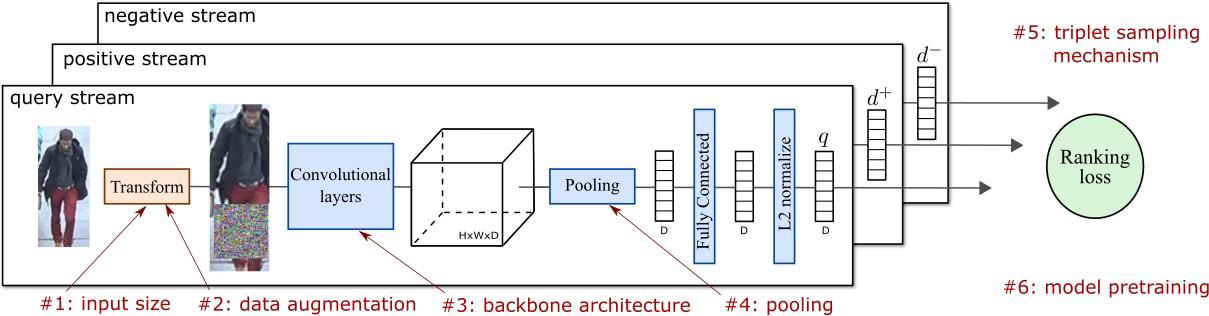
\includegraphics[width=0.8\linewidth]{images/siamese-net}
    \caption[Siamese network for person re-identification]{Siamese network for person re-identification}
    \label{fig:siamese-net}
\end{figure}

The base mechanism used by this net is called \textbf{Curriculum Learning}:
\begin{myitem}
    \item Pre-training for classification (ImageNet first, then classification - see step \#6);
    \item Increasingly difficult data transformation (image cut-out of increasing sizes - see step
    \#2);
    \item Hard triplet mining (see step \#5).
\end{myitem}

\textbf{Grad-CAM} highlights regions that activate dimensions in the resulting embeddings, so we can see which regions matter for matching image pairs, referring to the dimensions that contribute most to the similarity.

\begin{figure}[h!]
    \centering
    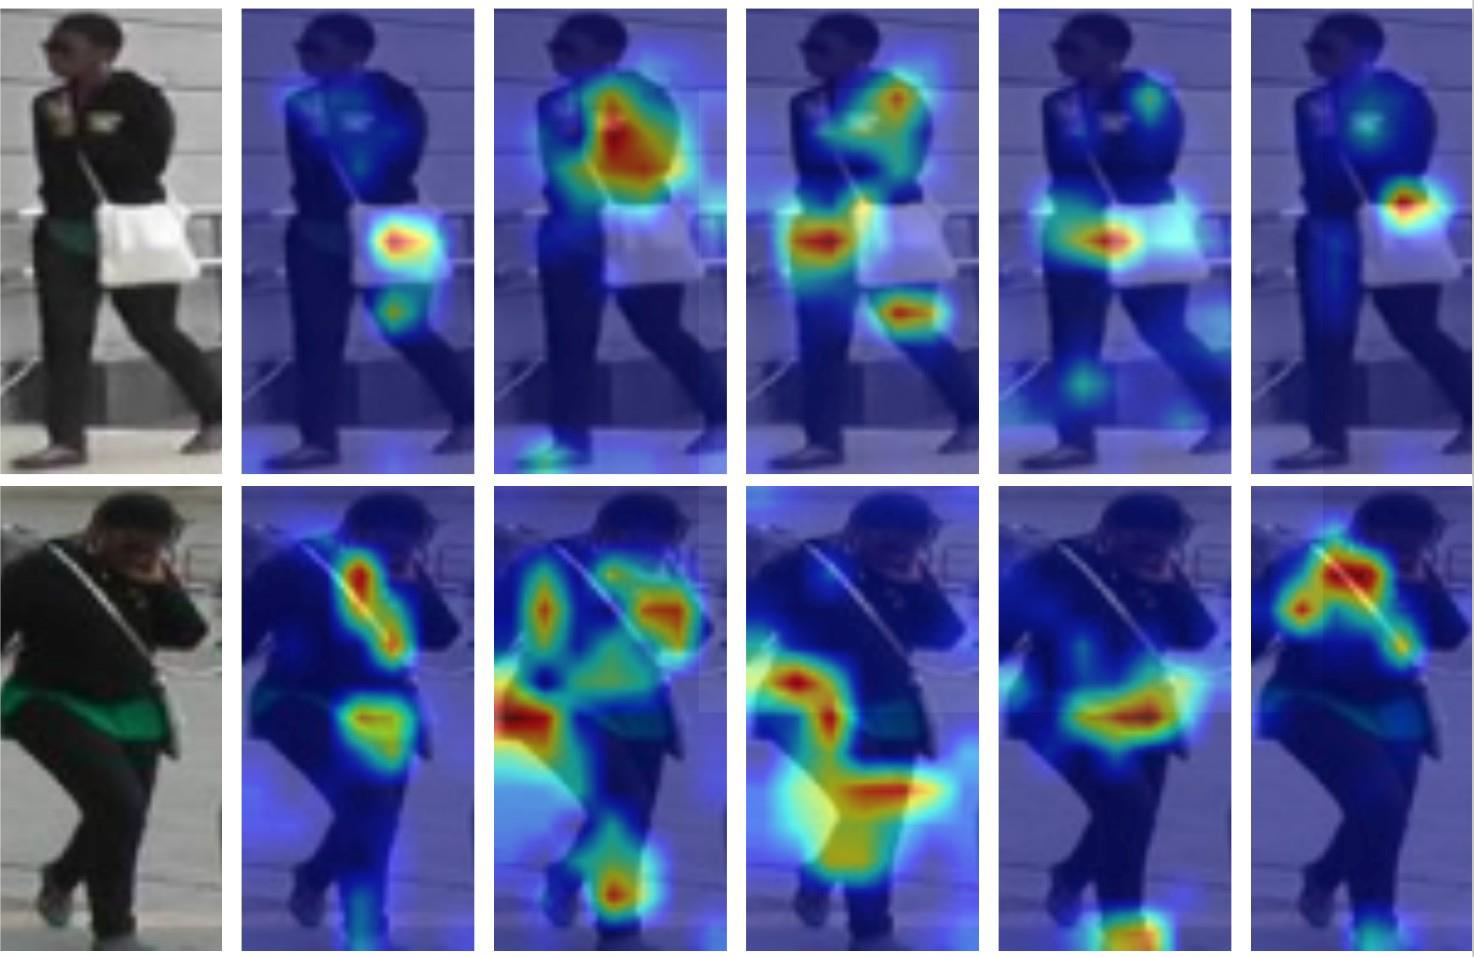
\includegraphics[width=0.6\linewidth]{images/grad-cam}
    \caption[Grad-CAM]{Grad-CAM}
    \label{fig:grad-cam}
\end{figure}



\subsubsection{Person Search}\label{sec:vs-person-search}

\textit{Sub-goal}: find a queried person within a gallery of images (detection + re-identification, without cropping gallery images).

This task is closer to actual applications such as missing persons or surveillance.

\begin{figure}[h!]
    \centering
    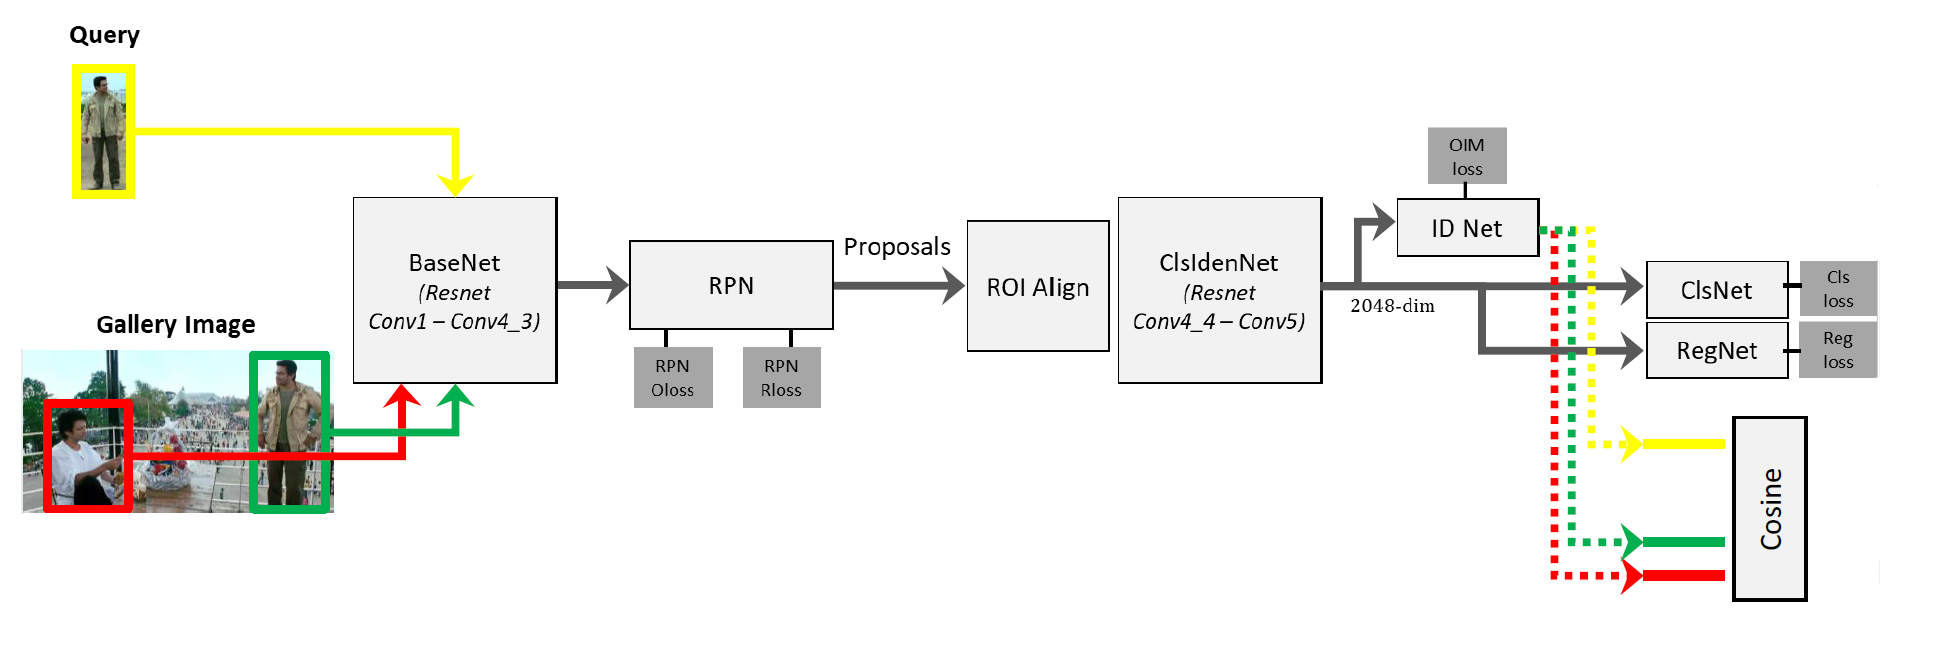
\includegraphics[width=.9\linewidth]{images/oim}
    \caption[OIM network]{OIM network}
    \label{fig:oim}
\end{figure}

The idea behind the \textbf{OIM} network (in figure \ref{fig:oim}) is to combine a \textit{Faster R-CNN} detection network to \textit{ID Net}, a network for re-identification vector embedding.\\
The objective of the network is to minimize the distance among features from the same identities and maximize those from different identities. The acronym OIM stands for the \textit{Online Instance Matching} lookup table, containing features of labeled and unlabeled identities, to compare against, and used for learning ID Net. Softmax converges slowly and needs more parameters with more identities.

Since the next model we will study uses this module, let's now introduce the  \textbf{Squeeze-and-Excitation Network} (SE-Net): it performs feature recalibration based on channel interdependencies, giving better results then ResNet on the ImageNet dataset. (See figures \ref{fig:se-net-1} and \ref{fig:se-net-2})

\begin{minipage}{.65\textwidth}
    \begin{figure}[H]
        \centering
        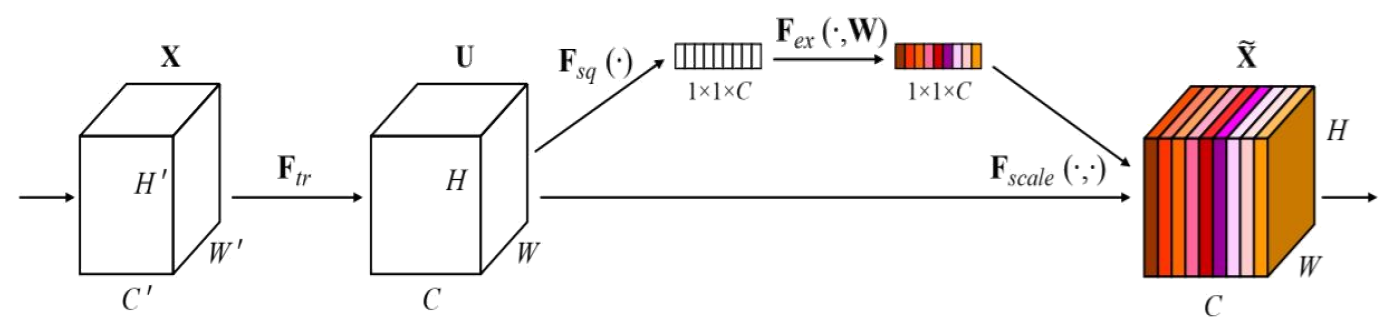
\includegraphics[width=.95\linewidth]{images/se-net-1}
        \caption[SE-Net]{SE-Net}
        \label{fig:se-net-1}
    \end{figure}
\end{minipage}
\begin{minipage}{.35\textwidth}
    \begin{figure}[H]
        \centering
        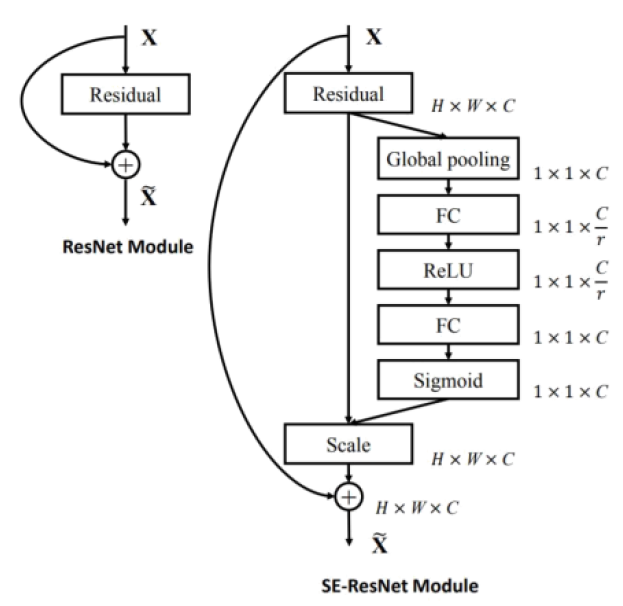
\includegraphics[width=.95\linewidth]{images/se-net-2}
        \caption[SE-Net vs ResNet]{SE-Net vs ResNet}
        \label{fig:se-net-2}
    \end{figure}
\end{minipage}

The principle on which \textbf{QEEPS} (Query-guided End-to-End Person Search) is based, is to use the query image extensively and learn end to end. That is, the query image is complete, not cropped, so that the network can use the context (e.g. illumination, colors, ...) to better distinguish the person we are looking for.\\
The architecture (see figure \ref{fig:qeeps}) is composed as follows:
\begin{myitem}
    \item \textit{Siamese Faster RCNN}: processes the query and gallery image in the same way and learns from the joint feedback;
    \item \textit{Re-ID network}: performs the re-identification part of the task;
    \item \textit{QSimNet} (see figure \ref{fig:qsimnet}): metric learning of re-identification vector distances, i.e., the similarity between the query image and the gallery image is determined using a NN instead of the cosine similarity (as in OIM);
    \item \textit{QRPN} (Query-guided RPN - see figure \ref{fig:qrpn}): query-specific person proposals;
    \item \textit{QSSE} (Query-guided Siamese SE-Net - see figure \ref{fig:qsse}): global-context guidance to the base net.
\end{myitem}

\begin{figure}[h!]
    \centering
    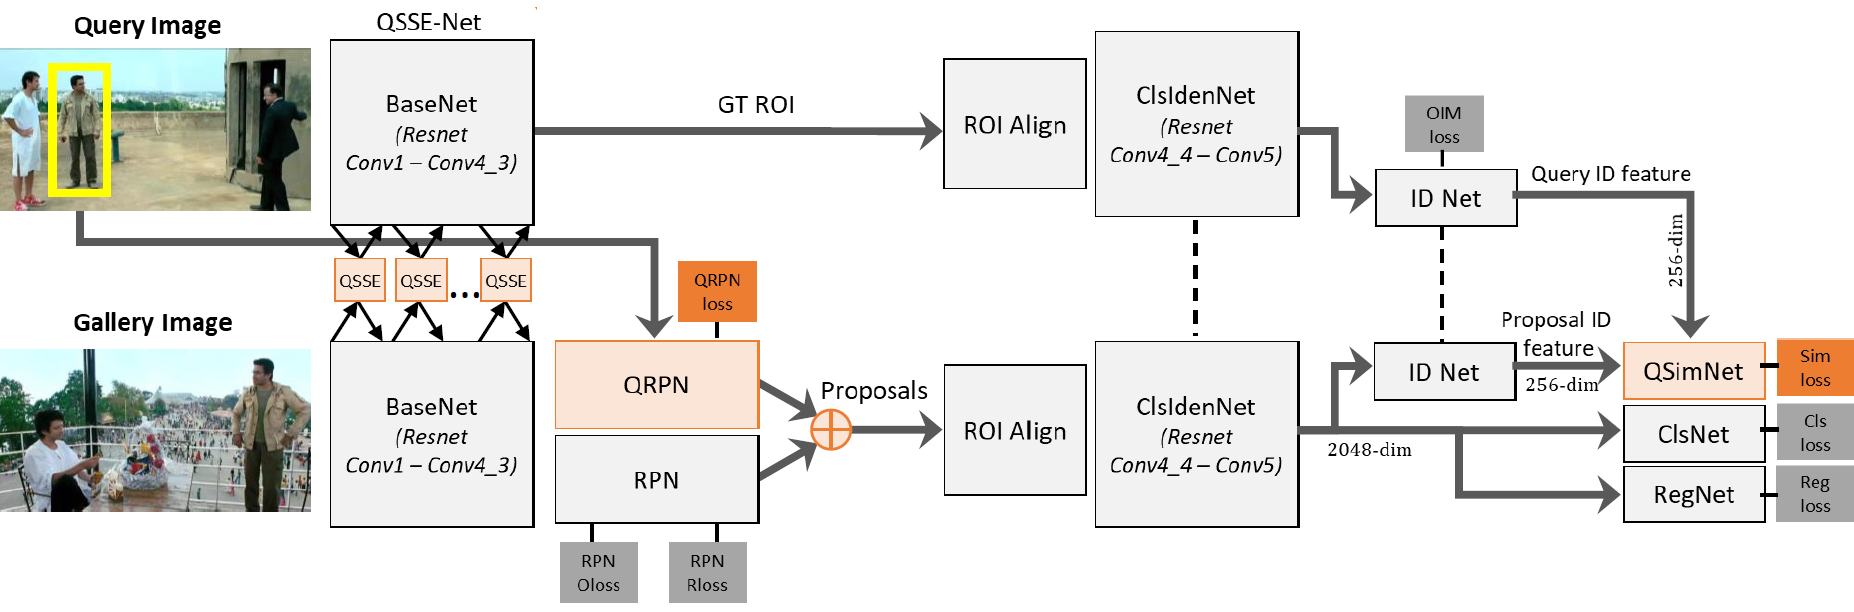
\includegraphics[width=.9\linewidth]{images/qeeps}
    \caption[QEEPS]{QEEPS}
    \label{fig:qeeps}
\end{figure}
\begin{minipage}{.35\textwidth}
    \begin{figure}[H]
        \centering
        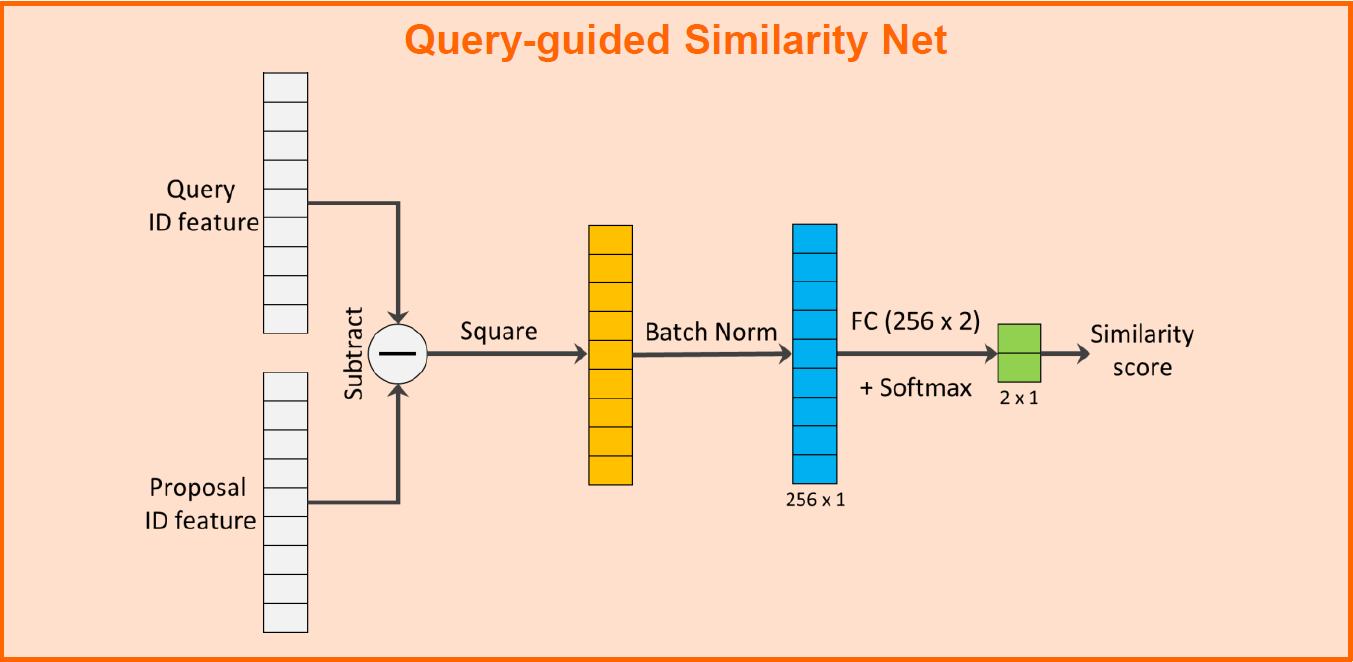
\includegraphics[width=.95\linewidth]{images/qsimnet}
        \caption[QSimNet]{QSimNet}
        \label{fig:qsimnet}
    \end{figure}
\end{minipage}
\begin{minipage}{.39\textwidth}
    \begin{figure}[H]
        \centering
        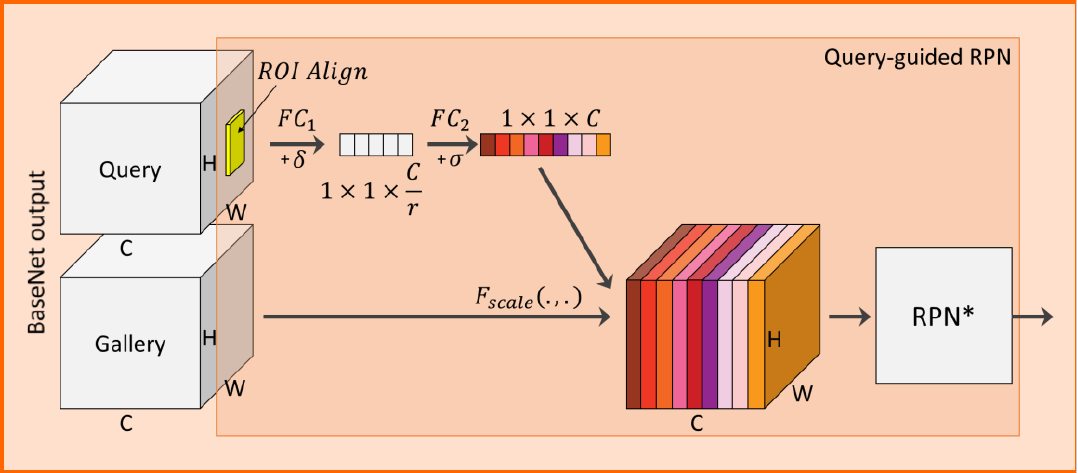
\includegraphics[width=.95\linewidth]{images/qrpn}
        \caption[QRPN]{QRPN}
        \label{fig:qrpn}
    \end{figure}
\end{minipage}
\begin{minipage}{.26\textwidth}
    \begin{figure}[H]
        \centering
        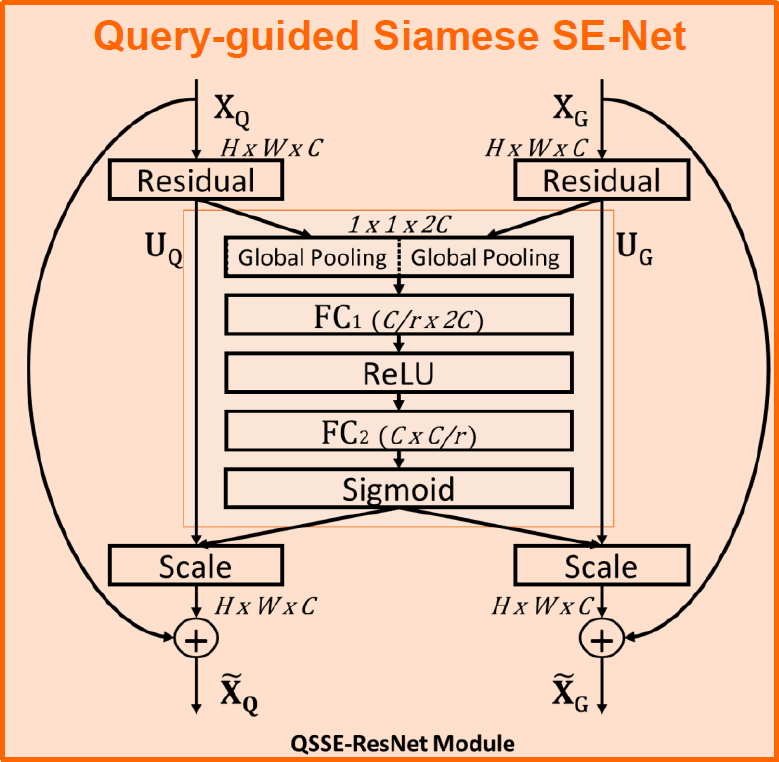
\includegraphics[width=.95\linewidth]{images/qsse}
        \caption[QSSE]{QSSE}
        \label{fig:qsse}
    \end{figure}
\end{minipage}

The corresponding overall loss function is computed as follows, as a combination of different losses:
\begin{equation}\label{eq:qeeps-loss}
    L = \underbrace{ \lambda_1 L_{cls} + \lambda_2 L_{reg} + \lambda_3 L_{rpn_o} + \lambda_4 L_{rpn_r} }_{\text{Faster R-CNN losses}} + \underbrace{ \lambda_5 L_{oim} }_{\text{OIM loss}} + \underbrace{ \lambda_6 L_{qrpn} }_{\text{QRPN loss}} + \underbrace{ \lambda_7 L_{sim} }_{\text{QSimNet loss}}
\end{equation}
where $L_{qrpn}$ and $L_{sim}$ are cross-entropy losses, i.e. $- \frac1N \sum_N \log(p_n^u)$, and QSSE Net gets the implicit same supervision as the BaseNet.

Evaluation:
\begin{myitem}
    \item \textit{Ablating the model parts}: incremental tests are performed by using only OIM first, then adding the other modules; the result is that QSimNet is the module that gives the most relevant performance improvement, but it is still useful to combine all the modules.
    \item \textit{Comparison to state-of-the art}: using larger image resolution gives state-of-the art performance, and in general this model gives consistent improvement across datasets and image resolutions.
    \item \textit{Qualitative results}: plotting the test images with the results given by QEEPS shows that it can distinguish even very similar persons, also in challenging conditions (e.g. from the back).
\end{myitem}


\subsection{Semantic Search}\label{sec:vs-semantic}

\textit{Goal}: mine patterns in large collections.

Queries can be complex and involve the full scene, instead of a single object as in Object Search (see section \ref{sec:vs-object}).

The intrinsic complexity of the task causes that even human annotations are difficult, since different annotators can give different descriptions of an image and its meaning. Thus, the evaluation si based on a leave-one-user-out agreement score: $89.1 \pm 4.6$.

An attempt to capture semantic information in images has been done with the \textit{Visual Genome dataset}, composed of thousands of images with millions of descriptions and object instances.

Practically speaking, the objective is to learn a compact visual representation for the semantic search task. Training data is composed of images with human captions, privileged information which can be leveraged as a proxy for semantic similarity. That, is: two image are semantically similar if their captions are similar. This idea can be applied to visual and textual representations: \textit{visual representations} of images with similar captions are close in the semantic embedding space, \textit{textual representations} of corresponding captions are close in the semantic embedding space.

To learn such a \textbf{semantic embedding}, we can use a Three-stream Siamese Network like the one used for deep representations in visual search (see figure \ref{fig:training-retrieval}, section \ref{sec:vs-deep}) and multiple losses similar to the previously cited triplet loss (see \ref{eq:retrieval-triplet-loss}):
\begin{flalign}\label{eq:semantic-triplet-loss}
    L_v(q,d^+,d^-) &= \frac12 \max(0, m - \phi_q^T \phi_+ + \phi_q^T \phi_-)\tag{Visual loss}\\
    L_{t1}(q,d^+,d^-) &= \frac12 \max(0, m - \phi_q^T \theta_+ + \phi_q^T \theta_-)\tag{Textual loss 1}\\
    L_{t2}(q,d^+,d^-) &= \frac12 \max(0, m - \theta_q^T \phi_+ + \theta_q^T \phi_-)\tag{Textual loss 2}
\end{flalign}
Possible evaluation metrics are:
\begin{myitem}
    \item \textit{Evaluation on the triplets}: User-based score (agreement score between visual predictions and users' ground truth);
    \item Evaluation on the full test set (agreement score between visual predictions and proxy ground truth, i.e. human-generated captions):
    \begin{itemize}
        \item NDCG: normalized discounted cumulative gain,
        \item PCC: Pearson's correlation coefficient.
    \end{itemize}
\end{myitem}

The joint embedding allows for multimodal queries.

To tackle more complex queries, it is useful to implicitly understand or explicitly model scenes.
